% pre-v1.tex
%
% Purpose:
%   Flowchart-style Beamer presentation of the theory part of the rewritten
%   draft on guided modes in line-defect periodic waveguides.  The method is
%   split into modules (Rayleigh ports, BIE solver, far-field extractor,
%   cell S-matrix, ordered QZ, center cell, NEP, scan, raw field, jump
%   evaluator, mass / trace constant, distance theorem, certified interval),
%   each shown as a box with its inputs, outputs and one key formula.
%
% Main workflow:
%   overall flow -> module map -> two theory slides -> one slide per module,
%   each with a "you are here" mini module map.
%
% Based on:
%   draft/tmp/theory-rewrite/*.tex (sections 1--5, appendix A) and
%   pre/pre-v1/archive/pre-v1.tex (text-heavy first version).
%
% Main differences:
%   Replaces the text-heavy archived version by box-and-arrow diagrams with
%   minimal text.  Numerical results are intentionally not included.
%
% Numerical goal:
%   None; presentation of the method structure only.

\documentclass[aspectratio=169]{beamer}

\usetheme{CambridgeUS}
\usecolortheme{dove}
\usefonttheme{professionalfonts}

\usepackage{amsmath}
\usepackage{amssymb}
\usepackage{mathrsfs}
\usepackage{stmaryrd}
\usepackage{bm}
\usepackage{etoolbox}
\usepackage{tikz}
\usetikzlibrary{arrows.meta,calc,decorations.pathreplacing,positioning,shapes.geometric}

\newcommand{\ii}{\mathrm{i}}
\newcommand{\ee}{\mathrm{e}}
\newcommand{\RR}{\mathbb{R}}
\newcommand{\jump}[1]{\llbracket #1\rrbracket}
\newcommand{\QP}{\mathrm{QP}}
\newcommand{\eps}{\varepsilon_{\partial}}
\newcommand{\dist}{\operatorname{dist}}

\setbeamertemplate{navigation symbols}{}
\setbeamertemplate{bibliography item}[text]

% Highlighted one-line statement.
\newcommand{\keybox}[1]{%
  \tikz\node[draw=red!60!black, line width=0.8pt, rounded corners=3pt,
    fill=red!4, inner sep=6pt, align=center]{#1};%
}

% ----------------------------------------------------------------------
% Diagram styles
% ----------------------------------------------------------------------
\tikzset{
  base/.style={rounded corners=3pt, draw, align=center, font=\scriptsize,
    minimum height=0.95cm, text width=1.6cm, line width=0.6pt},
  th/.style={base, fill=blue!10, draw=blue!60!black},
  cp/.style={base, fill=orange!14, draw=orange!75!black},
  ct/.style={base, fill=green!14, draw=green!45!black},
  io/.style={ellipse, draw=black!45, fill=gray!8, align=center,
    font=\scriptsize, inner sep=1.2pt},
  arr/.style={-{Latex[length=2mm]}, line width=0.7pt, draw=black!70},
  darr/.style={arr, dashed},
  big/.style={text width=2.6cm, minimum height=1.15cm, font=\small},
  hlif/.code 2 args={\ifstrequal{#1}{#2}{\pgfkeysalso{line width=1.8pt,
    draw=red!75!black, fill=red!20}}{}},
}

% Full module map; #1 = name of the module to highlight (or "none").
\newcommand{\modulemap}[1]{%
  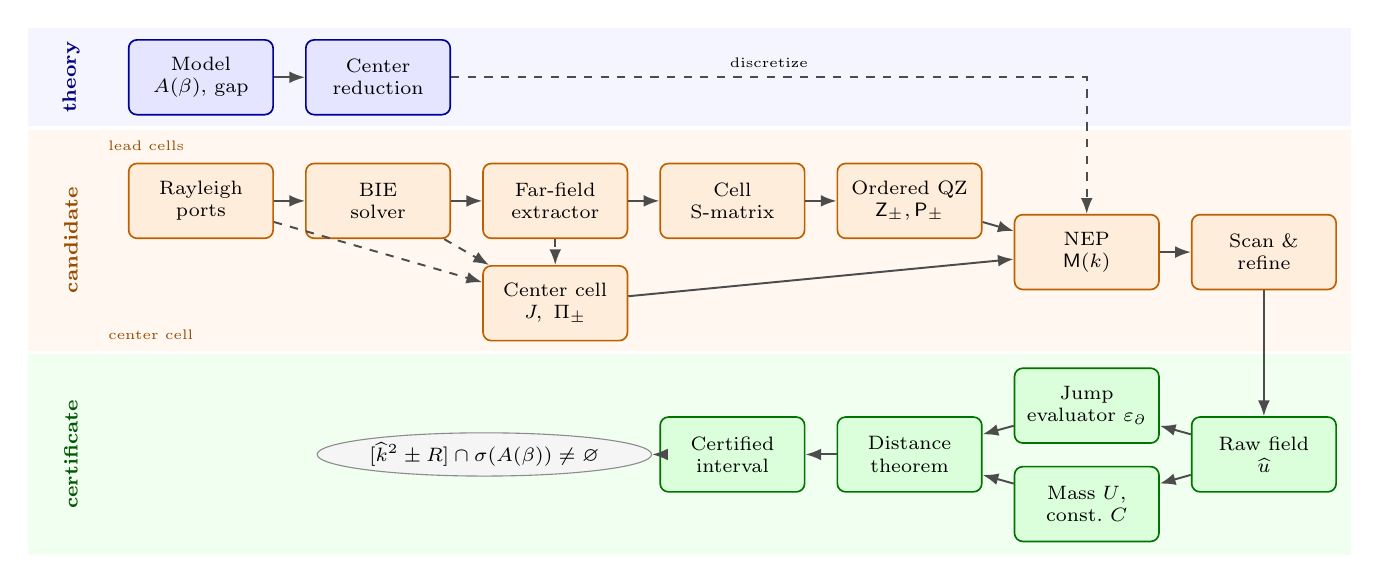
\begin{tikzpicture}[x=1cm,y=1cm]
    \fill[blue!4] (-2.2,3.0) rectangle (14.6,4.25);
    \fill[orange!6] (-2.2,0.15) rectangle (14.6,2.95);
    \fill[green!6] (-2.2,-2.45) rectangle (14.6,0.1);
    \node[rotate=90, font=\scriptsize\bfseries, blue!50!black] at (-1.65,3.62) {theory};
    \node[rotate=90, font=\scriptsize\bfseries, orange!60!black, align=center] at (-1.65,1.55) {candidate};
    \node[rotate=90, font=\scriptsize\bfseries, green!35!black] at (-1.65,-1.17) {certificate};
    \node[font=\tiny, orange!60!black, anchor=west] at (-1.3,2.75) {lead cells};
    \node[font=\tiny, orange!60!black, anchor=west] at (-1.3,0.35) {center cell};
    % theory
    \node[th, hlif={model}{#1}] (model) at (0,3.62) {Model\\$A(\beta)$, gap};
    \node[th, hlif={red}{#1}] (red) at (2.25,3.62) {Center\\reduction};
    % lead cells
    \node[cp, hlif={ray}{#1}] (ray) at (0,2.05) {Rayleigh\\ports};
    \node[cp, hlif={bie}{#1}] (bie) at (2.25,2.05) {BIE\\solver};
    \node[cp, hlif={ffe}{#1}] (ffe) at (4.5,2.05) {Far-field\\extractor};
    \node[cp, hlif={smat}{#1}] (smat) at (6.75,2.05) {Cell\\S-matrix};
    \node[cp, hlif={qz}{#1}] (qz) at (9.0,2.05) {Ordered QZ\\$\mathsf Z_\pm,\mathsf P_\pm$};
    % center cell
    \node[cp, hlif={ctr}{#1}] (ctr) at (4.5,0.75) {Center cell\\$J,\ \Pi_\pm$};
    \node[cp, hlif={nep}{#1}] (nep) at (11.25,1.4) {NEP\\$\mathsf M(k)$};
    \node[cp, hlif={scan}{#1}] (scan) at (13.5,1.4) {Scan \&\\refine};
    % certificate
    \node[ct, hlif={raw}{#1}] (raw) at (13.5,-1.17) {Raw field\\$\widehat u$};
    \node[ct, hlif={jump}{#1}] (jump) at (11.25,-0.55) {Jump\\evaluator $\eps$};
    \node[ct, hlif={mass}{#1}] (mass) at (11.25,-1.8) {Mass $U$,\\const.\ $C$};
    \node[ct, hlif={thm}{#1}] (thm) at (9.0,-1.17) {Distance\\theorem};
    \node[ct, hlif={cert}{#1}] (cert) at (6.75,-1.17) {Certified\\interval};
    \node[io] (out) at (3.6,-1.17) {$[\widehat k^2\pm R]\cap\sigma(A(\beta))\neq\varnothing$};
    % arrows
    \draw[arr] (model) -- (red);
    \draw[darr] (red.east) -- (11.25,3.62) node[pos=0.5, above, font=\tiny] {discretize} -- (nep.north);
    \draw[arr] (ray) -- (bie);
    \draw[arr] (bie) -- (ffe);
    \draw[arr] (ffe) -- (smat);
    \draw[arr] (smat) -- (qz);
    \draw[arr] (qz) -- (nep);
    \draw[darr] (ray) -- (ctr);
    \draw[darr] (bie) -- (ctr);
    \draw[darr] (ffe) -- (ctr);
    \draw[arr] (ctr) -- (nep);
    \draw[arr] (nep) -- (scan);
    \draw[arr] (scan) -- (raw);
    \draw[arr] (raw) -- (jump);
    \draw[arr] (raw) -- (mass);
    \draw[arr] (jump) -- (thm);
    \draw[arr] (mass) -- (thm);
    \draw[arr] (thm) -- (cert);
    \draw[arr] (cert) -- (out);
  \end{tikzpicture}%
}

% "You are here" mini map at the bottom right of a [t] frame.
\newsavebox{\mmbox}
\newcommand{\minimap}[1]{%
  \sbox{\mmbox}{\resizebox{0.22\paperwidth}{!}{\modulemap{#1}}}%
  \begin{tikzpicture}[remember picture, overlay]
    \node[anchor=south east, inner sep=0pt, draw=black!25]
      at ($(current page.south east)+(-0.2,0.45)$) {\usebox{\mmbox}};
  \end{tikzpicture}%
}

\title[Guided modes: method map]{Guided Modes in Line-Defect Periodic Waveguides}
\subtitle{A module map of the method (theory, pre-v1)}
\author{}
\date{}

\begin{document}

\begin{frame}
  \titlepage
\end{frame}

% ======================================================================
\section{Overview}

\begin{frame}{The whole idea in one picture}
  \centering
  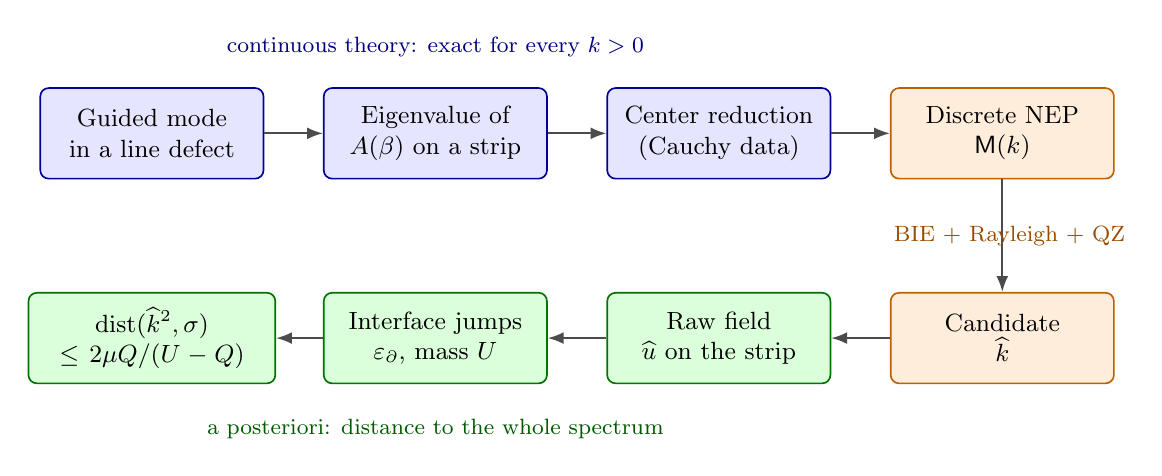
\begin{tikzpicture}[x=1cm,y=1cm]
    \node[th, big] (a) at (0,0) {Guided mode\\in a line defect};
    \node[th, big] (b) at (3.6,0) {Eigenvalue of\\$A(\beta)$ on a strip};
    \node[th, big] (c) at (7.2,0) {Center reduction\\(Cauchy data)};
    \node[cp, big] (d) at (10.8,0) {Discrete NEP\\$\mathsf M(k)$};
    \node[cp, big] (e) at (10.8,-2.6) {Candidate\\$\widehat k$};
    \node[ct, big] (f) at (7.2,-2.6) {Raw field\\$\widehat u$ on the strip};
    \node[ct, big] (g) at (3.6,-2.6) {Interface jumps\\$\eps$, mass $U$};
    \node[ct, big, text width=2.9cm] (h) at (0,-2.6)
      {$\dist(\widehat k^2,\sigma)$\\$\le2\mu Q/(U-Q)$};
    \draw[arr] (a) -- (b);
    \draw[arr] (b) -- (c);
    \draw[arr] (c) -- (d);
    \draw[arr] (d) -- (e);
    \draw[arr] (e) -- (f);
    \draw[arr] (f) -- (g);
    \draw[arr] (g) -- (h);
    \node[font=\footnotesize, blue!50!black] at (3.6,1.1) {continuous theory: exact for every $k>0$};
    \node[font=\footnotesize, orange!60!black, anchor=west] at (9.3,-1.3) {BIE + Rayleigh + QZ};
    \node[font=\footnotesize, green!35!black] at (3.6,-3.75) {a posteriori: distance to the whole spectrum};
  \end{tikzpicture}
\end{frame}

\begin{frame}{Module map}
  \centering
  \resizebox{\textwidth}{!}{\modulemap{none}}

  \vspace{0.5em}
  \footnotesize
  \tikz\node[th, minimum height=0.3cm, text width=0.3cm]{};~theory\quad
  \tikz\node[cp, minimum height=0.3cm, text width=0.3cm]{};~candidate computation\quad
  \tikz\node[ct, minimum height=0.3cm, text width=0.3cm]{};~certificate\quad
  dashed: reused module
\end{frame}

% ======================================================================
\section{Theory}

\begin{frame}[t]{Model: line defect $\to$ $A(\beta)$}
  \centering
  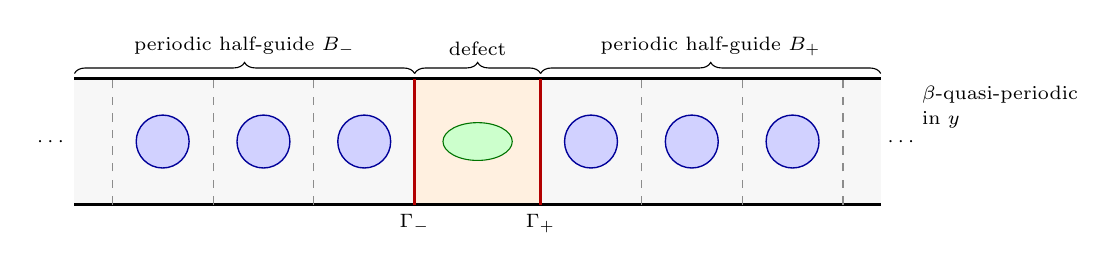
\begin{tikzpicture}[x=0.8cm,y=0.8cm, every node/.style={font=\scriptsize},
      incl/.style={draw=blue!60!black, fill=blue!18, line width=0.5pt}]
    \fill[gray!6] (-6.4,-1) rectangle (6.4,1);
    \fill[orange!12] (-1,-1) rectangle (1,1);
    \draw[thick] (-6.4,1) -- (6.4,1);
    \draw[thick] (-6.4,-1) -- (6.4,-1);
    \foreach \x in {-5.8,-4.2,-2.6,2.6,4.2,5.8} \draw[black!45, dashed] (\x,-1) -- (\x,1);
    \draw[red!70!black, line width=1.1pt] (-1,-1) -- (-1,1);
    \draw[red!70!black, line width=1.1pt] (1,-1) -- (1,1);
    \foreach \c in {1.8,3.4,5.0,-1.8,-3.4,-5.0} \draw[incl] (\c,0) circle (0.42);
    \draw[draw=green!45!black, fill=green!20] (0,0) ellipse (0.55 and 0.3);
    \node at (6.75,0) {$\cdots$};
    \node at (-6.75,0) {$\cdots$};
    \node[below] at (-1,-1) {$\Gamma_-$};
    \node[below] at (1,-1) {$\Gamma_+$};
    \draw[decorate, decoration={brace, amplitude=4pt}] (-6.4,1.08) -- (-1,1.08)
      node[midway, above=3pt] {periodic half-guide $B_-$};
    \draw[decorate, decoration={brace, amplitude=4pt}] (-1,1.08) -- (1,1.08)
      node[midway, above=3pt] {defect};
    \draw[decorate, decoration={brace, amplitude=4pt}] (1,1.08) -- (6.4,1.08)
      node[midway, above=3pt] {periodic half-guide $B_+$};
    \node[right] at (6.9,0.75) {$\beta$-quasi-periodic};
    \node[right] at (6.9,0.35) {in $y$};
  \end{tikzpicture}

  \vspace{0.6em}
  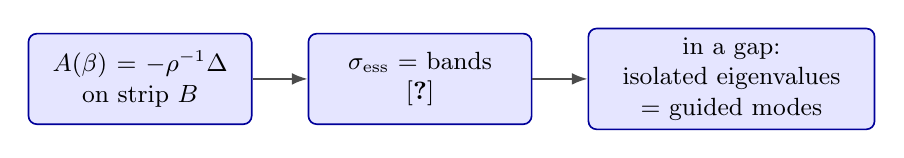
\begin{tikzpicture}[node distance=0.7cm]
    \node[th, big] (a) {$A(\beta)=-\rho^{-1}\Delta$\\on strip $B$};
    \node[th, big, right=of a] (b) {$\sigma_{\mathrm{ess}}$ = bands\\\cite{Fliss2013}};
    \node[th, big, right=of b, text width=3.4cm] (c) {in a gap:\\isolated eigenvalues\\= guided modes};
    \draw[arr] (a) -- (b);
    \draw[arr] (b) -- (c);
  \end{tikzpicture}
  \minimap{model}
\end{frame}

\begin{frame}[t]{Center reduction via Cauchy data}
  \centering
  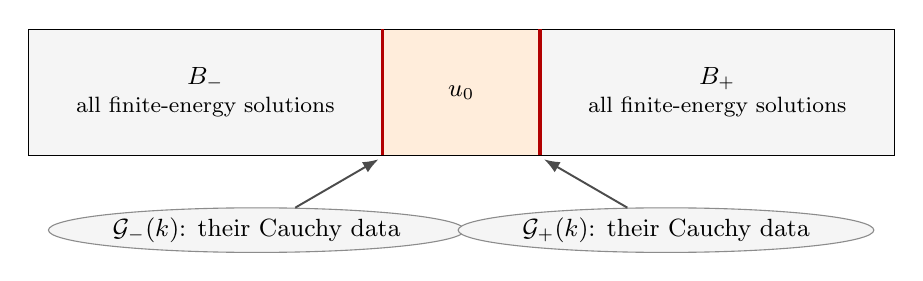
\begin{tikzpicture}[x=1cm,y=1cm, every node/.style={font=\small}]
    \fill[gray!8] (-5.5,-0.8) rectangle (-1,0.8);
    \fill[orange!14] (-1,-0.8) rectangle (1,0.8);
    \fill[gray!8] (1,-0.8) rectangle (5.5,0.8);
    \draw (-5.5,-0.8) rectangle (5.5,0.8);
    \draw[red!70!black, line width=1.2pt] (-1,-0.8) -- (-1,0.8);
    \draw[red!70!black, line width=1.2pt] (1,-0.8) -- (1,0.8);
    \node[align=center] at (-3.25,0) {$B_-$\\[-1pt]{\footnotesize all finite-energy solutions}};
    \node at (0,0) {$u_0$};
    \node[align=center] at (3.25,0) {$B_+$\\[-1pt]{\footnotesize all finite-energy solutions}};
    \node[io, font=\small] (gm) at (-2.6,-1.75) {$\mathcal G_-(k)$: their Cauchy data};
    \node[io, font=\small] (gp) at (2.6,-1.75) {$\mathcal G_+(k)$: their Cauchy data};
    \draw[arr] (gm) -- (-1.05,-0.85);
    \draw[arr] (gp) -- (1.05,-0.85);
  \end{tikzpicture}

  \vspace{0.6em}
  \keybox{guided mode at $k$ \quad$\Longleftrightarrow$\quad
    $u_0\neq0$ solves the center problem and
    $(u_0,\partial_\nu u_0)|_{\Gamma_\pm}\in\mathcal G_\pm(k)$}

  \vspace{0.4em}
  \small
  Exact for every $k>0$. DtN \cite{Fliss2013} is the special case where $\mathcal G_\pm$ is a graph.
  \minimap{red}
\end{frame}

% ======================================================================
\section{Candidate computation}

\begin{frame}[t]{Module: Rayleigh ports}
  \centering
  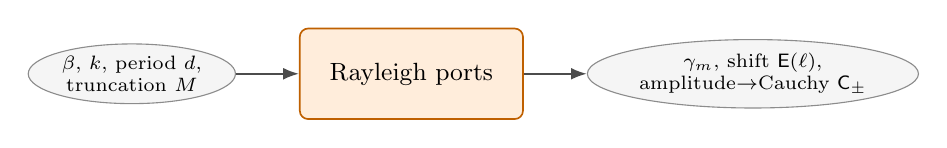
\begin{tikzpicture}[node distance=0.8cm]
    \node[io] (i) {$\beta$, $k$, period $d$,\\truncation $M$};
    \node[cp, big, right=of i] (m) {Rayleigh ports};
    \node[io, right=of m] (o) {$\gamma_m$, shift $\mathsf E(\ell)$,\\amplitude$\to$Cauchy $\mathsf C_\pm$};
    \draw[arr] (i) -- (m);
    \draw[arr] (m) -- (o);
  \end{tikzpicture}

  \vspace{1em}
  In a homogeneous strip, every solution is a sum of right/left-going waves:
  \[
    u=\sum_m\bigl(a_m\,\ee^{\ii\gamma_m(x-x_p)}+b_m\,\ee^{-\ii\gamma_m(x-x_p)}\bigr)\psi_m(y),
    \qquad
    \begin{bmatrix}u\\ \partial_\nu u\end{bmatrix}_m=\mathsf C_\pm\begin{bmatrix}a\\ b\end{bmatrix}.
  \]
  \centering\small
  Common language for all ports: amplitudes $(a,b)$.
  \minimap{ray}
\end{frame}

\begin{frame}[t]{Module: BIE solver}
  \centering
  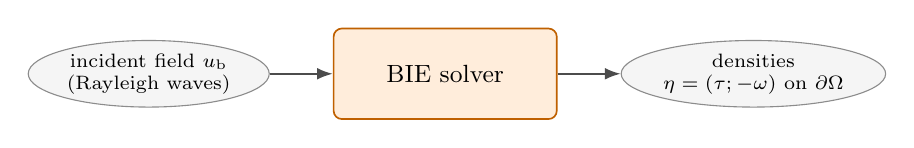
\begin{tikzpicture}[node distance=0.8cm]
    \node[io] (i) {incident field $u_{\mathrm b}$\\(Rayleigh waves)};
    \node[cp, big, right=of i] (m) {BIE solver};
    \node[io, right=of m] (o) {densities\\$\eta=(\tau;-\omega)$ on $\partial\Omega$};
    \draw[arr] (i) -- (m);
    \draw[arr] (m) -- (o);
  \end{tikzpicture}

  \vspace{1em}
  \[
    \mathscr J_k[\eta;u_{\mathrm b}]
    =\begin{bmatrix}\text{value jump}\\ \text{normal-derivative jump}\end{bmatrix}_{\partial\Omega}=0
  \]
  \small
  QP layer potentials outside, free-space inside.\\
  Second-kind system, Kress--Nystr\"om \cite{Kress1991,DominguezLyonTurc2016}.
  \minimap{bie}
\end{frame}

\begin{frame}[t]{Module: far-field extractor}
  \centering
  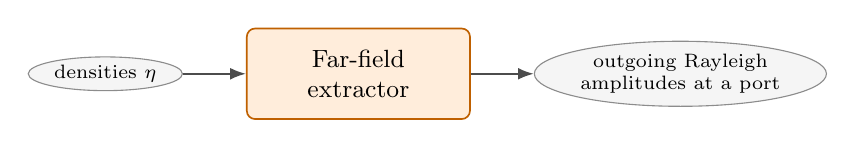
\begin{tikzpicture}[node distance=0.8cm]
    \node[io] (i) {densities $\eta$};
    \node[cp, big, right=of i] (m) {Far-field\\extractor};
    \node[io, right=of m] (o) {outgoing Rayleigh\\amplitudes at a port};
    \draw[arr] (i) -- (m);
    \draw[arr] (m) -- (o);
  \end{tikzpicture}

  \vspace{0.6em}
  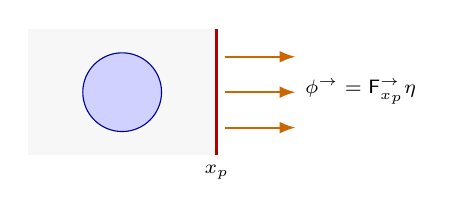
\begin{tikzpicture}[x=1cm,y=1cm]
    \fill[gray!6] (0,-0.8) rectangle (2.4,0.8);
    \draw[draw=blue!60!black, fill=blue!18] (1.2,0) circle (0.5);
    \draw[red!70!black, line width=1.1pt] (2.4,-0.8) -- (2.4,0.8);
    \node[font=\scriptsize, below] at (2.4,-0.8) {$x_p$};
    \foreach \y in {-0.45,0,0.45} \draw[arr, orange!80!black] (2.5,\y) -- (3.4,\y);
    \node[font=\scriptsize, right] at (3.4,0) {$\phi^{\rightarrow}=\mathsf F^{\rightarrow}_{x_p}\eta$};
  \end{tikzpicture}

  \vspace{0.4em}
  \small
  Read off directly from the spectral series of $G_\QP$ \cite{Linton1998}; no port
  sampling or FFT.
  \minimap{ffe}
\end{frame}

\begin{frame}[t]{Module: cell S-matrix}
  \centering
  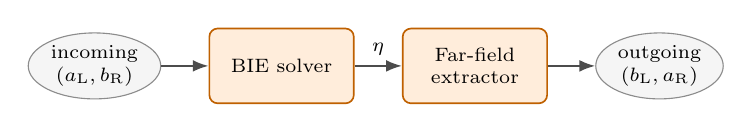
\begin{tikzpicture}[node distance=0.6cm]
    \node[io] (i) {incoming\\$(a_{\mathrm L},b_{\mathrm R})$};
    \node[cp, right=of i] (m1) {BIE solver};
    \node[cp, right=of m1] (m2) {Far-field\\extractor};
    \node[io, right=of m2] (o) {outgoing\\$(b_{\mathrm L},a_{\mathrm R})$};
    \draw[arr] (i) -- (m1);
    \draw[arr] (m1) -- node[above, font=\scriptsize] {$\eta$} (m2);
    \draw[arr] (m2) -- (o);
  \end{tikzpicture}

  \vspace{0.5em}
  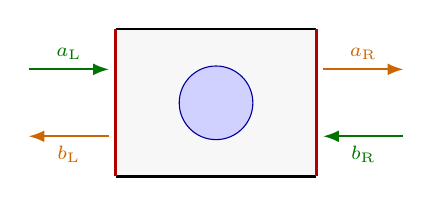
\begin{tikzpicture}[x=0.85cm,y=0.85cm, every node/.style={font=\scriptsize}]
    \fill[gray!6] (0,-1.1) rectangle (3,1.1);
    \draw[thick] (0,1.1) -- (3,1.1);
    \draw[thick] (0,-1.1) -- (3,-1.1);
    \draw[red!70!black, line width=1.1pt] (0,-1.1) -- (0,1.1);
    \draw[red!70!black, line width=1.1pt] (3,-1.1) -- (3,1.1);
    \draw[draw=blue!60!black, fill=blue!18] (1.5,0) circle (0.55);
    \draw[arr, green!45!black] (-1.3,0.5) -- (-0.1,0.5) node[midway, above] {$a_{\mathrm L}$};
    \draw[arr, orange!80!black] (-0.1,-0.5) -- (-1.3,-0.5) node[midway, below] {$b_{\mathrm L}$};
    \draw[arr, green!45!black] (4.3,-0.5) -- (3.1,-0.5) node[midway, below] {$b_{\mathrm R}$};
    \draw[arr, orange!80!black] (3.1,0.5) -- (4.3,0.5) node[midway, above] {$a_{\mathrm R}$};
  \end{tikzpicture}

  \[
    \begin{bmatrix}b_{\mathrm L}\\ a_{\mathrm R}\end{bmatrix}
    =\begin{bmatrix}R_{\mathrm L}&T_{\mathrm{RL}}\\ T_{\mathrm{LR}}&R_{\mathrm R}\end{bmatrix}
    \begin{bmatrix}a_{\mathrm L}\\ b_{\mathrm R}\end{bmatrix}
  \]
  \minimap{smat}
\end{frame}

\begin{frame}[t]{Module: ordered QZ}
  \centering
  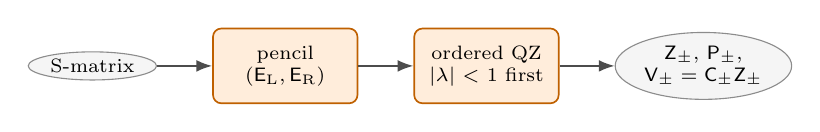
\begin{tikzpicture}[node distance=0.7cm]
    \node[io] (i) {S-matrix};
    \node[cp, right=of i] (m1) {pencil\\$(\mathsf E_{\mathrm L},\mathsf E_{\mathrm R})$};
    \node[cp, right=of m1] (m2) {ordered QZ\\$|\lambda|<1$ first};
    \node[io, right=of m2] (o) {$\mathsf Z_\pm$, $\mathsf P_\pm$,\\$\mathsf V_\pm=\mathsf C_\pm\mathsf Z_\pm$};
    \draw[arr] (i) -- (m1);
    \draw[arr] (m1) -- (m2);
    \draw[arr] (m2) -- (o);
  \end{tikzpicture}

  \vspace{0.3em}
  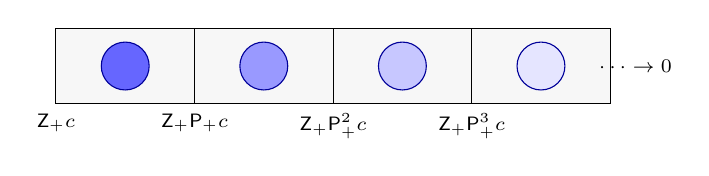
\begin{tikzpicture}[x=0.8cm,y=0.8cm, every node/.style={font=\scriptsize}]
    \foreach \j/\o in {0/60,1/40,2/22,3/10} {
      \fill[gray!6] (2.2*\j,-0.6) rectangle (2.2*\j+2.2,0.6);
      \draw (2.2*\j,-0.6) rectangle (2.2*\j+2.2,0.6);
      \draw[draw=blue!60!black, fill=blue!\o] (2.2*\j+1.1,0) circle (0.38);
    }
    \node[below] at (0,-0.6) {$\mathsf Z_+c$};
    \node[below] at (2.2,-0.6) {$\mathsf Z_+\mathsf P_+c$};
    \node[below] at (4.4,-0.6) {$\mathsf Z_+\mathsf P_+^2c$};
    \node[below] at (6.6,-0.6) {$\mathsf Z_+\mathsf P_+^3c$};
    \node at (9.2,0) {$\cdots\to0$};
  \end{tikzpicture}

  \[
    \mathsf E_{\mathrm L}\mathsf Z_+=\mathsf E_{\mathrm R}\mathsf Z_+\mathsf P_+,\qquad
    \rho(\mathsf P_+)<1
  \]
  \small
  Decaying family $\Rightarrow$ $\operatorname{range}\mathsf V_\pm\approx\mathcal G_\pm(k)$
  \cite{JolyLiFliss2006}.
  \minimap{qz}
\end{frame}

\begin{frame}[t]{Module: center cell}
  \centering
  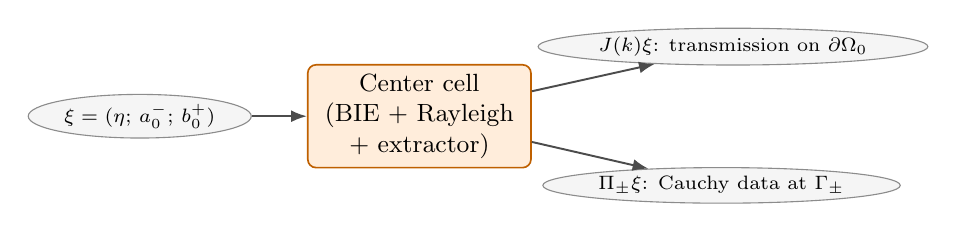
\begin{tikzpicture}[node distance=0.7cm]
    \node[io] (i) {$\xi=(\eta;\,a_0^-;\,b_0^+)$};
    \node[cp, big, right=of i] (m) {Center cell\\(BIE + Rayleigh\\+ extractor)};
    \node[io, above right=0.05cm and 0.8cm of m] (o1) {$J(k)\xi$: transmission on $\partial\Omega_0$};
    \node[io, below right=0.05cm and 0.8cm of m] (o2) {$\Pi_\pm\xi$: Cauchy data at $\Gamma_\pm$};
    \draw[arr] (i) -- (m);
    \draw[arr] (m) -- (o1);
    \draw[arr] (m) -- (o2);
  \end{tikzpicture}

  \[
    u=\underbrace{\mathcal S_\QP[\omega]+\mathcal D_\QP[\tau]}_{\text{outgoing at both ports}}
    +\underbrace{\textstyle\sum_m\bigl(a^-_{0,m}r_m^{x_-}+b^+_{0,m}l_m^{x_+}\bigr)}_{u_{\mathrm{hom}}:\ \text{incoming}}
  \]
  \small
  $u_{\mathrm{hom}}$ is needed even without a center inclusion.
  \minimap{ctr}
\end{frame}

\begin{frame}[t]{Module: NEP assembly}
  \centering
  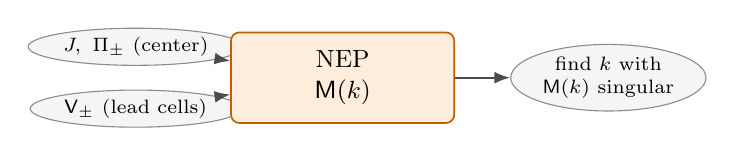
\begin{tikzpicture}[node distance=0.7cm]
    \node[io] (i1) {$J,\ \Pi_\pm$ (center)};
    \node[io, below=0.3cm of i1] (i2) {$\mathsf V_\pm$ (lead cells)};
    \node[cp, big, right=1.2cm of $(i1)!0.5!(i2)$] (m) {NEP\\$\mathsf M(k)$};
    \node[io, right=of m] (o) {find $k$ with\\$\mathsf M(k)$ singular};
    \draw[arr] (i1) -- (m);
    \draw[arr] (i2) -- (m);
    \draw[arr] (m) -- (o);
  \end{tikzpicture}

  \vspace{0.6em}
  \[
    \mathsf M(k)=
    \left[\begin{array}{c|cc}
      J & 0 & 0\\
      \Pi_- & -\mathsf V_- & 0\\
      \Pi_+ & 0 & -\mathsf V_+
    \end{array}\right]
    \begin{array}{l}
      \leftarrow\ \text{transmission on }\partial\Omega_0\\
      \leftarrow\ \text{Cauchy data at }\Gamma_-\in\operatorname{range}\mathsf V_-\\
      \leftarrow\ \text{Cauchy data at }\Gamma_+\in\operatorname{range}\mathsf V_+
    \end{array}
  \]
  \small
  Unknowns $(\xi;c_-;c_+)$. This is the discrete center reduction.
  \minimap{nep}
\end{frame}

\begin{frame}[t]{Module: scan \& refine}
  \centering
  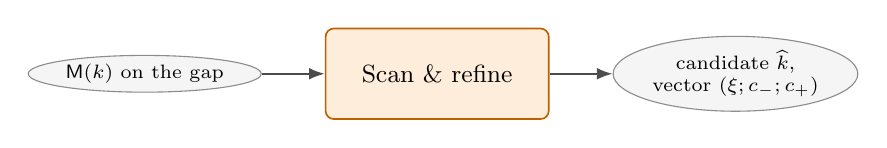
\begin{tikzpicture}[node distance=0.8cm]
    \node[io] (i) {$\mathsf M(k)$ on the gap};
    \node[cp, big, right=of i] (m) {Scan \& refine};
    \node[io, right=of m] (o) {candidate $\widehat k$,\\vector $(\xi;c_-;c_+)$};
    \draw[arr] (i) -- (m);
    \draw[arr] (m) -- (o);
  \end{tikzpicture}

  \vspace{0.4em}
  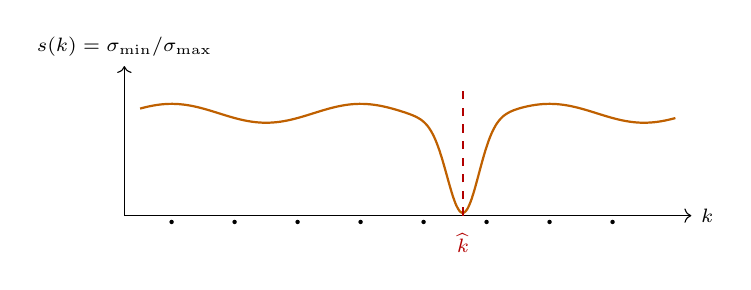
\begin{tikzpicture}[x=1cm,y=1cm]
    \draw[->] (0,0) -- (7.2,0) node[right, font=\scriptsize] {$k$};
    \draw[->] (0,0) -- (0,1.9) node[above, font=\scriptsize] {$s(k)=\sigma_{\min}/\sigma_{\max}$};
    \draw[thick, orange!75!black, domain=0.2:7, samples=150, smooth]
      plot (\x, {1.3-1.15*exp(-((\x-4.3)/0.28)^2)+0.12*sin(150*\x)});
    \foreach \x in {0.6,1.4,...,6.8} \fill (\x,-0.08) circle (0.8pt);
    \draw[red!70!black, dashed] (4.3,0) -- (4.3,1.6);
    \node[red!70!black, below, font=\scriptsize] at (4.3,-0.1) {$\widehat k$};
  \end{tikzpicture}

  \small
  Small $s(\widehat k)$ $\neq$ error bound $\Rightarrow$ certify.
  \minimap{scan}
\end{frame}

% ======================================================================
\section{Certificate}

\begin{frame}[t]{Module: raw field}
  \centering
  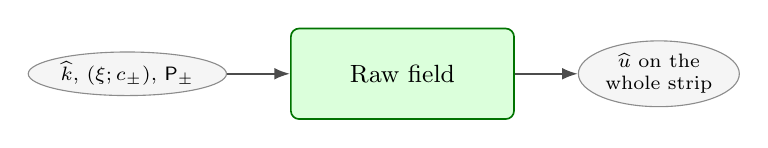
\begin{tikzpicture}[node distance=0.8cm]
    \node[io] (i) {$\widehat k$, $(\xi;c_\pm)$, $\mathsf P_\pm$};
    \node[ct, big, right=of i] (m) {Raw field};
    \node[io, right=of m] (o) {$\widehat u$ on the\\whole strip};
    \draw[arr] (i) -- (m);
    \draw[arr] (m) -- (o);
  \end{tikzpicture}

  \vspace{0.6em}
  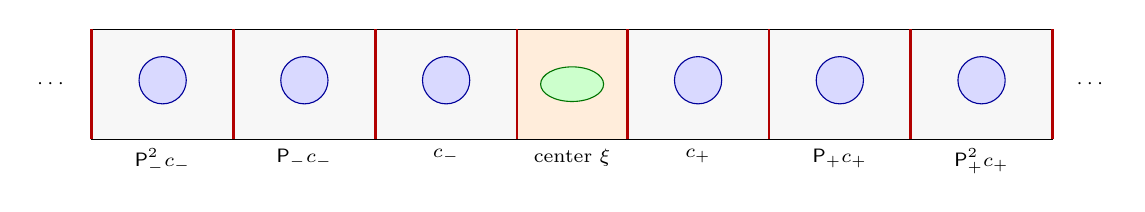
\begin{tikzpicture}[x=1cm,y=1cm, every node/.style={font=\scriptsize}]
    \foreach \x/\l in {-5.2/{\mathsf P_-^2c_-},-3.4/{\mathsf P_-c_-},-1.6/{c_-},1.6/{c_+},3.4/{\mathsf P_+c_+},5.2/{\mathsf P_+^2c_+}} {
      \fill[gray!6] (\x-0.9,-0.7) rectangle (\x+0.9,0.7);
      \draw (\x-0.9,-0.7) rectangle (\x+0.9,0.7);
      \draw[draw=blue!60!black, fill=blue!15] (\x,0.05) circle (0.3);
      \node[below] at (\x,-0.7) {$\l$};
    }
    \fill[orange!14] (-0.7,-0.7) rectangle (0.7,0.7);
    \draw (-0.7,-0.7) rectangle (0.7,0.7);
    \draw[draw=green!45!black, fill=green!20] (0,0) ellipse (0.4 and 0.22);
    \node[below] at (0,-0.7) {center $\xi$};
    \foreach \x in {-6.1,-4.3,-2.5,-0.7,0.7,2.5,4.3,6.1}
      \draw[red!70!black, line width=1pt] (\x,-0.7) -- (\x,0.7);
    \node at (6.6,0) {$\cdots$};
    \node at (-6.6,0) {$\cdots$};
  \end{tikzpicture}

  \vspace{0.3em}
  \small
  Exact Helmholtz in every piece.\\
  Errors live \emph{only} as jumps on interfaces.
  \minimap{raw}
\end{frame}

\begin{frame}[t]{Module: jump evaluator}
  \centering
  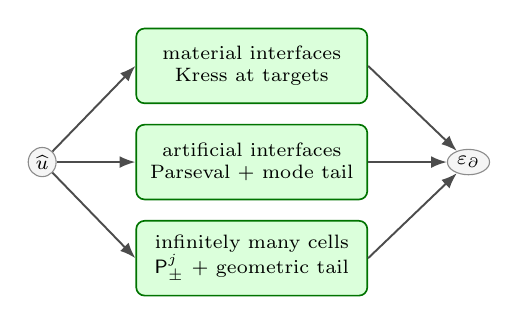
\begin{tikzpicture}[node distance=0.5cm]
    \node[io] (i) {$\widehat u$};
    \node[ct, text width=2.7cm, right=1cm of i] (m2) {artificial interfaces\\Parseval + mode tail};
    \node[ct, text width=2.7cm, above=0.25cm of m2] (m1) {material interfaces\\Kress at targets};
    \node[ct, text width=2.7cm, below=0.25cm of m2] (m3) {infinitely many cells\\$\mathsf P_\pm^j$ + geometric tail};
    \node[io, right=1cm of m2] (o) {$\eps$};
    \foreach \m in {m1,m2,m3} {\draw[arr] (i) -- (\m.west); \draw[arr] (\m.east) -- (o);}
  \end{tikzpicture}

  \[
    \eps^2=\sum_{\text{all interfaces }\Gamma}
    \Bigl(\lVert\jump{\partial_\nu\widehat u}\rVert_{L^2(\Gamma)}^2
      +\ell_*^{-2}\lVert\jump{\widehat u}\rVert_{L^2(\Gamma)}^2\Bigr)
  \]
  \small
  Infinite sums = finite part + rigorous tails.
  \minimap{jump}
\end{frame}

\begin{frame}[t]{Module: mass and trace constant}
  \centering
  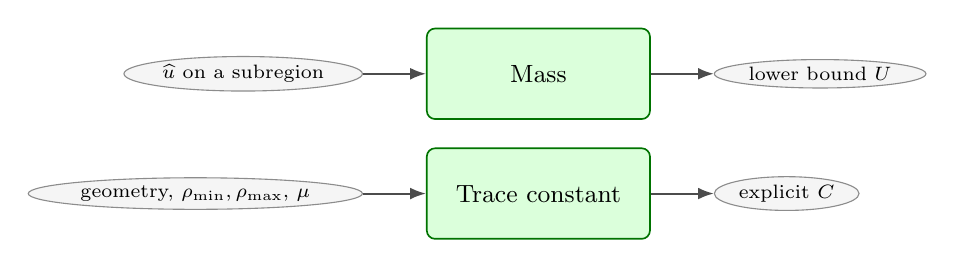
\begin{tikzpicture}[node distance=0.8cm]
    \node[io] (i1) {$\widehat u$ on a subregion};
    \node[ct, big, right=of i1] (m1) {Mass};
    \node[io, right=of m1] (o1) {lower bound $U$};
    \draw[arr] (i1) -- (m1);
    \draw[arr] (m1) -- (o1);
    \node[ct, big, below=0.35cm of m1] (m2) {Trace constant};
    \node[io, left=of m2] (i2) {geometry, $\rho_{\min},\rho_{\max}$, $\mu$};
    \node[io, right=of m2] (o2) {explicit $C$};
    \draw[arr] (i2) -- (m2);
    \draw[arr] (m2) -- (o2);
  \end{tikzpicture}

  \[
    \sum_\Gamma\Bigl(\lVert v\rVert_{L^2(\Gamma)}^2+\ell_*^2\lVert\partial_\nu v\rVert_{L^2(\Gamma)}^2\Bigr)
    \le C^2\,\lVert(A(\beta)+\mu)v\rVert^2
  \]
  \small
  No fitting to residuals.
  \minimap{mass}
\end{frame}

\begin{frame}[t]{Module: distance theorem}
  \centering
  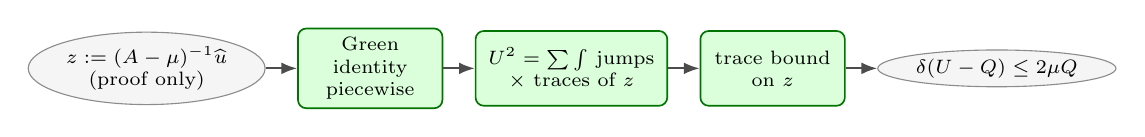
\begin{tikzpicture}[node distance=0.4cm]
    \node[io] (a) {$z:=(A-\mu)^{-1}\widehat u$\\(proof only)};
    \node[ct, right=of a] (b) {Green identity\\piecewise};
    \node[ct, right=of b, text width=2.2cm] (c) {$U^2=\sum\int$ jumps\\$\times$ traces of $z$};
    \node[ct, right=of c] (d) {trace bound\\on $z$};
    \node[io, right=of d] (e) {$\delta(U-Q)\le2\mu Q$};
    \draw[arr] (a) -- (b);
    \draw[arr] (b) -- (c);
    \draw[arr] (c) -- (d);
    \draw[arr] (d) -- (e);
  \end{tikzpicture}

  \vspace{1.2em}
  \keybox{$Q:=C\,\eps<U\quad\Longrightarrow\quad
    \displaystyle\dist\bigl(\widehat k^2,\sigma(A(\beta))\bigr)\le\frac{2\mu Q}{U-Q}$}

  \vspace{0.8em}
  \small
  Distance to the whole spectrum: no prior gap check needed (cf.\ \cite{BarnettHassellTacy2018}).
  \minimap{thm}
\end{frame}

\begin{frame}[t]{Module: certified interval}
  \centering
  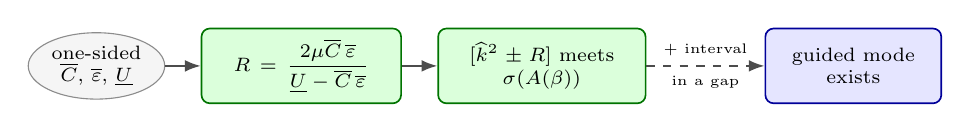
\begin{tikzpicture}[node distance=0.45cm]
    \node[io] (a) {one-sided\\$\overline C$, $\overline\varepsilon$, $\underline U$};
    \node[ct, right=of a, text width=2.3cm] (b) {$R=\dfrac{2\mu\overline C\,\overline\varepsilon}{\underline U-\overline C\,\overline\varepsilon}$};
    \node[ct, right=of b, text width=2.4cm] (c) {$[\widehat k^2\pm R]$ meets\\$\sigma(A(\beta))$};
    \node[th, right=1.5cm of c, text width=2.0cm] (d) {guided mode\\exists};
    \draw[arr] (a) -- (b);
    \draw[arr] (b) -- (c);
    \draw[darr] (c) -- node[above, font=\tiny] {+ interval} node[below, font=\tiny] {in a gap} (d);
  \end{tikzpicture}

  \vspace{1.5em}
  \small
  Every input is a one-sided bound from the \emph{same} $\widehat u$.\\[0.3em]
  Not claimed: index, multiplicity, uniqueness, a priori convergence.
  \minimap{cert}
\end{frame}

% ======================================================================
\section{Summary}

\begin{frame}{Summary}
  \centering
  \resizebox{0.95\textwidth}{!}{\modulemap{none}}

  \vspace{0.6em}
  \small
  Exact reduction $\to$ modular BIE computation $\to$ a posteriori certificate.\\
  Next: numerical results.
\end{frame}

\begin{frame}{References}
  \tiny
  \bibliographystyle{plain}
  \bibliography{../../ref/reference}
\end{frame}

\end{document}
